
\section{Opaque without survivability}\label{ILP_Opaque_Survivability}

\subsection{Model description}

In order to be able to apply the ILP model we have to take into account the physical and logical topologies allowed by this mode of transport and the type of survivability. Based on what was mentioned in section \ref{opaque} on this mode of transport we can conclude that both topologies are the same and the following figures can be confirmed.\\

\begin{figure}[h!]
\centering
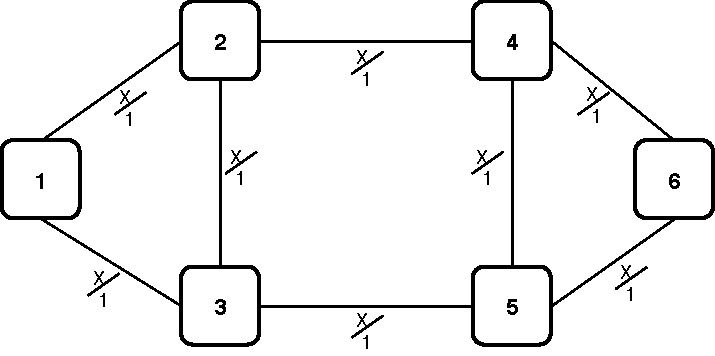
\includegraphics[width=10cm]{sdf/ilp/opaque_survivability/figures/allowed_physical_topology}
\caption{Opaque without survivability: allowed physical topology. The allowed physical topology is defined by the duct and sites in the field. It is assumed that each duct supports up to 1 bidirectional transmission system and each site supports up to 1 node.}
\label{allowed_physical_low}
\end{figure}

\newpage
\begin{figure}[h!]
\centering
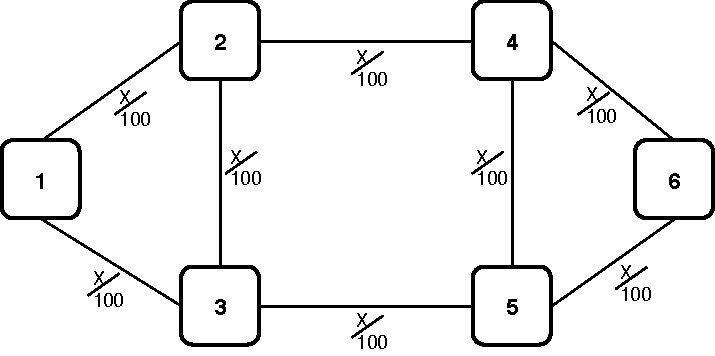
\includegraphics[width=10cm]{sdf/ilp/opaque_survivability/figures/allowed_optical_topology}
\caption{Opaque without survivability: allowed optical topology. The allowed optical topology is defined by the transport mode. It is assumed that each transmission system supports up to 100 optical channels.}
\label{allowed_optical_low}
\end{figure}

Now taking this into account and based on the specific constraints of the opaque mode without survivability it is possible to define the ILP model \cite{aularui}.\\

The objective function, to be minimized, is the expression \ref{Capex},

\begin{equation}
  minimize \qquad \Big\{ \quad C_C \quad \Big\}
  \label{ILPOpaque_CAPEX}
\end{equation}

$subject$ $to$
\begin{equation}
\sum_{j=1\textbackslash \{o\}}^{N} fb_{ij}^{od} = 1  \qquad \qquad \qquad \qquad \qquad \qquad \qquad \qquad \qquad
\forall(o,d) : o < d, \forall i: i = o
\label{ILPOpaque1_Surv}
\end{equation}
\noindent
Constraint \ref{ILPOpaque1_Surv} is equal to the constraint \ref{ILPOpaque1_CAPEX} assuming that Z = 1.

\begin{equation}
\sum_{j=1\textbackslash \{o\}}^{N} fb_{ij}^{od} = \sum_{j=1\textbackslash \{d\}}^{N} f_{ji}^{od}   \qquad \qquad \qquad \qquad \qquad \qquad
\forall(o,d) : o < d, \forall i: i \neq o,d
\label{ILPOpaque2_Surv}
\end{equation}
\noindent
Constraint \ref{ILPOpaque2_Surv} is equal to the constraint \ref{ILPOpaque2_CAPEX}.

\begin{equation}
\sum_{j=1\textbackslash \{d\}}^{N} fb_{ji}^{od} = 1  \qquad \qquad \qquad \qquad \qquad \qquad \qquad \qquad \qquad
\forall(o,d) : o < d, \forall i: i = d
\label{ILPOpaque3_Surv}
\end{equation}
\noindent
Constraint \ref{ILPOpaque3_Surv} is equal to the constraint \ref{ILPOpaque3_CAPEX} assuming that Z = 1.

\begin{equation}
\sum_{o=1}^{N} \sum_{d=o+1}^{N} \left(fb_{ij}^{od} + fb_{ji}^{od}\right) \sum_{c=1}^{C} (B\left(c\right) D_{odc})\leq \tau W_{ij} G_{ij} \qquad \qquad \qquad \qquad
\forall(i,j) : i < j
\label{ILPOpaque4_Surv}
\end{equation}
\noindent
The constraint \ref{ILPOpaque4_Surv} is considered the grooming constraint, so it means that the total client traffic flows can not be greater than the capacity of the line bit rate. Where $\tau$ is the line bit rate. In this work we assume that $\tau$ = 100 Gbits/s. $G_{ij}$ is the adjacency matrix, which means that we can only use a connection if it exists in the physical topology of the network.

\begin{equation}
W_{ij} \leq K_{ij} L_{ij} \qquad  \qquad \qquad \qquad \qquad \qquad \qquad \qquad \qquad \qquad \qquad \qquad \forall(i,j) : i < j
\label{ILPOpaque5_Surv}
\end{equation}
\noindent
Constraint \ref{ILPOpaque5_Surv} concerns the capacity of the optical channels which must be less or equal than the maximum number of optical channels. For any situation the maximum number of optical channels supported by each transmission system is 100, i.e., $K_{ij}$ = 100.

\begin{equation}
fb_{ij}^{od} , fb_{ji}^{od}, L_{ij} \in \{0,1\}   \qquad \qquad \qquad \qquad \qquad \qquad \qquad
\forall(i,j) : i < j, \forall(o,d) : o < d
\label{ILPOpaque6_Surv}
\end{equation}
\noindent
Constraint \ref{ILPOpaque6_Surv} define the variables $fb$ and $L_{ij}$ as binary values.

\begin{equation}
W_{ij} \in \mathbb{N}  \qquad \qquad \qquad \qquad \qquad \qquad \qquad \qquad \qquad \qquad \qquad \qquad \qquad
\forall(i,j) : i < j
\label{ILPOpaque7_Surv}
\end{equation}
\noindent
This constraint defines the variables $W_{ij}$ as integer variables allowing that between each pair of nodes can exist more that one lightpath.

\subsection{Result description}

\textbf{Low Traffic Scenario:}\\

In a first phase, we will show the resulting physical and optical topology. These topologies are based on the allowed topologies referred to in the model description and also taking into account the logical topology for all ODUs mentioned in the section \ref{low_scenario}.

\begin{figure}[h!]
\centering
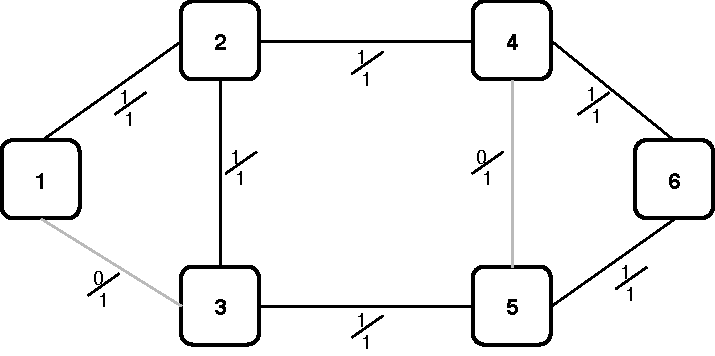
\includegraphics[width=11cm]{sdf/ilp/opaque_survivability/figures/physical_topology_low}
\caption{Opaque without survivability in low scenario: physical topology after dimensioning.}
\label{physical_low}
\end{figure}
\newpage
\begin{figure}[h!]
\centering
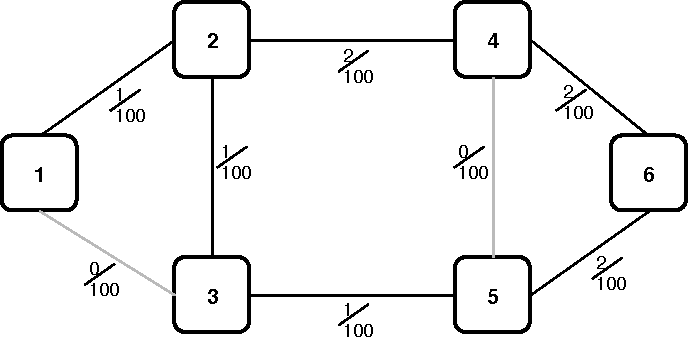
\includegraphics[width=11cm]{sdf/ilp/opaque_survivability/figures/optical_topology_low}
\caption{Opaque without survivability in low scenario: optical topology after dimensioning.}
\label{optical_low}
\end{figure}

In table \ref{link_opaque_surv_ref_low} we can see the number of optical channels calculated using \ref{Capex_Link} and \ref{ILPOpaque_CAPEX} and the number of amplifiers for each link calculated using \ref{Capex_amplifiers}. In the case where there are no optical channels we assume that the number of amplifiers is zero.

\begin{table}[h!]
\centering
\begin{tabular}{|| c | c | c ||}
 \hline
 \multicolumn{3}{|| c ||}{Information regarding links} \\
 \hline
 \hline
 Bidirectional Link & Optical Channels & Amplifiers\\
 \hline
 Node 1 <-> Node 2 & 1 & 4 \\
 Node 1 <-> Node 3 & 0 & 0 \\
 Node 2 <-> Node 3 & 1 & 0 \\
 Node 2 <-> Node 4 & 2 & 6 \\
 Node 3 <-> Node 5 & 1 & 8 \\
 Node 4 <-> Node 5 & 0 & 0 \\
 Node 4 <-> Node 6 & 2 & 7 \\
 Node 5 <-> Node 6 & 2 & 3 \\
 \hline
\end{tabular}
\caption{Table with information regarding links for opaque mode without survivability in low scenario.}
\label{link_opaque_surv_ref_low}
\end{table}

In table \ref{node_opaque_surv_ref_low} we can see the resulting nodal degree at the physical layer, calculated based on the number of connections that the node in question performs, the number of line ports calculated using \ref{EXC_pexc1_opaque} and the number of tributary ports calculated using \ref{EXC_pexc2_opaque} for each node.

\begin{table}[h!]
\centering
\begin{tabular}{|| c | c | c | c ||}
 \hline
 \multicolumn{4}{|| c ||}{Information regarding nodes} \\
 \hline
 \hline
 Node & Resulting Nodal Degree & Line Ports & Tributary Ports\\
 \hline
 1 & 1 & 1 & 29 \\
 2 & 3 & 4 & 23 \\
 3 & 2 & 2 & 18 \\
 4 & 2 & 4 & 20 \\
 5 & 2 & 3 & 24 \\
 6 & 2 & 4 & 22 \\
\hline
\end{tabular}
\caption{Table with information regarding nodes for opaque mode without survivability in low scenario.}
\label{node_opaque_surv_ref_low}
\end{table}

\newpage
Through the information obtained previously on the nodes we can now create tables with detailed information about each node. In each table mentioned below we can see how many ports are connected to a given node and its bit rate (in relation to the line ports) and how many ports are assigned to each different bit rate (in relation to the tributary ports).

\begin{table}[h!]
\centering
\begin{tabular}{|| c | c | c ||}
 \hline
 \multicolumn{3}{|| c ||}{Detailed description of Node 1} \\
 \hline
 \hline
  & Number of total demands & Bit rate \\
 \hline
 \multirow{3}{*}{29 tributary ports} & 13 & ODU0 \\
 & 13 & ODU1 \\
 & 3 & ODU2 \\
 \hline
 \hline
  & Node<--Optical Channels-->Node & Bit rate \\
 \hline
 1 line ports & 1  <---- 1 ---->  2 & 100 Gbits/s \\
\hline
\end{tabular}
\caption{Opaque without survivability in low scenario: detailed description of node 1. The number of demands is distributed to the various destination nodes, and can be observed in section \ref{low_scenario}.}
\end{table}

\begin{table}[h!]
\centering
\begin{tabular}{|| c | c | c ||}
 \hline
 \multicolumn{3}{|| c ||}{Detailed description of Node 2} \\
 \hline
 \hline
  & Number of total demands & Bit rate \\ \hline
 \multirow{5}{*}{23 tributary ports} & 11 & ODU0 \\
 & 7 & ODU1 \\
 & 2 & ODU2 \\
 & 2 & ODU3 \\
 & 1 & ODU4 \\
 \hline
 \hline
  & Node<--Optical Channels-->Node & Bit rate \\ \hline
 \multirow{3}{*}{4 line ports} & 2  <---- 1 ---->  1 & \multirow{3}{*}{100 Gbits/s} \\
 & 2  <---- 1 ---->  3 & \\
 & 2  <---- 2 ---->  4 & \\
\hline
\end{tabular}
\caption{Opaque without survivability in low scenario: detailed description of node 2. The number of demands is distributed to the various destination nodes, and can be observed in section \ref{low_scenario}.}
\end{table}

\begin{table}[h!]
\centering
\begin{tabular}{|| c | c | c ||}
 \hline
 \multicolumn{3}{|| c ||}{Detailed description of Node 3} \\
 \hline
 \hline
  & Number of total demands & Bit rate \\ \hline
 \multirow{4}{*}{18 tributary ports} & 7 & ODU0 \\
 & 6 & ODU1\\
 & 3 & ODU2\\
 & 2 & ODU3\\
 \hline
 \hline
  & Node<--Optical Channels-->Node & Bit rate \\
 \hline
 \multirow{2}{*}{2 line ports} & 3  <---- 1 ---->  2 & \multirow{2}{*}{100 Gbits/s}\\
 & 3  <---- 1 ---->  5 & \\
\hline
\end{tabular}
\caption{Opaque without survivability in low scenario: detailed description of node 3. The number of demands is distributed to the various destination nodes, and can be observed in section \ref{low_scenario}.}
\end{table}

\newpage
\begin{table}[h!]
\centering
\begin{tabular}{|| c | c | c ||}
 \hline
 \multicolumn{3}{|| c ||}{Detailed description of Node 4} \\
 \hline
 \hline
  & Number of total demands & Bit rate \\ \hline
 \multirow{3}{*}{20 tributary ports} & 7 & ODU0 \\
 & 10 & ODU1 \\
 & 3 & ODU2 \\
 \hline
 \hline
  & Node<--Optical Channels-->Node & Bit rate \\
 \hline
 \multirow{2}{*}{4 line ports} & 4  <---- 2 ---- >  2 & \multirow{2}{*}{100 Gbits/s}\\
 & 4  <---- 2 ----> 6 & \\
\hline
\end{tabular}
\caption{Opaque without survivability in low scenario: detailed description of node 4. The number of demands is distributed to the various destination nodes, and can be observed in section \ref{low_scenario}.}
\end{table}

\begin{table}[h!]
\centering
\begin{tabular}{|| c | c | c ||}
 \hline
 \multicolumn{3}{|| c ||}{Detailed description of Node 5} \\
 \hline
 \hline
  & Number of total demands & Bit rate \\ \hline
 \multirow{5}{*}{24 tributary ports} & 14 & ODU0 \\
 & 4 & ODU1 \\
 & 4 & ODU2 \\
 & 1 & ODU3 \\
 & 1 & ODU4 \\
 \hline
 \hline
  & Node<--Optical Channels-->Node & Bit rate \\
 \hline
 \multirow{2}{*}{3 line ports} & 5  <---- 1 ---->  3 & \multirow{2}{*}{100 Gbits/s}\\
 & 5  <---- 2 ---->  6 & \\
 \hline
\end{tabular}
\caption{Opaque without survivability in low scenario: detailed description of node 5. The number of demands is distributed to the various destination nodes, and can be observed in section \ref{low_scenario}.}
\end{table}

\begin{table}[h!]
\centering
\begin{tabular}{|| c | c | c ||}
 \hline
 \multicolumn{3}{|| c ||}{Detailed description of Node 6} \\
 \hline
 \hline
  & Number of total demands & Bit rate \\
 \hline
 \multirow{5}{*}{22 tributary ports} & 8 & ODU0 \\
 & 10 & ODU1 \\
 & 1 & ODU2 \\
 & 1 & ODU3 \\
 & 2 & ODU4 \\
 \hline
 \hline
  & Node<--Optical Channels-->Node & Bit rate \\
 \hline
 \multirow{2}{*}{4 line ports} & 6  <---- 2 ---->  4 & \multirow{2}{*}{100 Gbits/s}\\
 & 6  <---- 2 ---->  5 & \\
\hline
\end{tabular}
\caption{Opaque without survivability in low scenario: detailed description of node 6. The number of demands is distributed to the various destination nodes, and can be observed in section \ref{low_scenario}.}
\end{table}

\vspace{15pt}
In next step let's focus on the routing information. These paths are bidirectional so the path from one node to another is the same path in the opposite direction. In table \ref{path_opaque_surv_ref_low} we can see all the routing obtained for all nodes.\\
\newpage
\begin{table}[h!]
\centering
\begin{tabular}{|| c | c | c | c | c | c | c | c ||}
 \hline
 \multicolumn{8}{|| c ||}{Routing} \\
 \hline
 \hline
 o & d & Links & ODU0 & ODU1 & ODU2 & ODU3 & ODU4 \\
 \hline
 1 & 2 & \{(1,2)\} & 5 & 2 & 1 & 0 & 0 \\ \hline
 1 & 3 & \{(1,2),(2,3)\} & 1 & 4 & 1 & 0 & 0\\ \hline
 1 & 4 & \{(1,2),(2,4)\} & 3 & 2 & 1 & 0 & 0\\ \hline
 1 & 5 & \{(1,2),(2,3),(3,5)\} & 1 & 0 & 0 & 0 & 0\\ \hline
 1 & 6 & \{(1,2),(2,4),(4,6)\} & 3 & 5 & 0 & 0 & 0\\ \hline
 2 & 3 & \{(2,3)\} & 0 & 0 & 0 & 1 & 0 \\ \hline
 2 & 4 & \{(2,4)\} & 1 & 3 & 0 & 0 & 0\\ \hline
 2 & 5 & \{(2,3),(3,5)\} & 5 & 1 & 1 & 0 & 0 \\ \hline
 2 & 6 & \{(2,4),(4,6)\} & 0 & 1 & 0 & 1 & 1 \\ \hline
 3 & 4 & \{(3,2),(2,4)\} & 1 & 1 & 1 & 0 & 0 \\ \hline
 3 & 5 & \{(3,5)\} & 4 & 1 & 1 & 1 & 0 \\ \hline
 3 & 6 & \{(3,5),(5,6)\} & 1 & 0 & 0 & 0 & 0\\ \hline
 4 & 5 & \{(4,6),(6,5)\} & 1 & 1 & 1 & 0 & 0\\ \hline
 4 & 6 & \{(4,6)\} & 1 & 3 & 0 & 0 & 0\\ \hline
 5 & 6 & \{(5,6)\} & 3 & 1 & 1 & 0 & 1\\
 \hline
\end{tabular}
\caption{Opaque without survivability in low scenario: description of demands routing. We are assuming that between a pair of nodes all demands follow the same route.}
\label{path_opaque_surv_ref_low}
\end{table}

Finally and most importantly through table \ref{scriptopaque_surv_ref_low} we can see the CAPEX result for this model. All the values calculated in the next table were obtained through the equations \ref{Capex_Link} and \ref{Capex_Node} referred to in section \ref{ILP_CAPEX}.

\begin{table}[h!]
\centering
\begin{tabular}{||c|c|c|c|c|c|c||}
 \hline
 \multicolumn{7}{||c||}{CAPEX of the Network} \\
 \hline
 \hline
 \multicolumn{3}{||c|}{ }&Quantity&Unit Price&Cost&Total \\
 \hline
 \multirow{3}{*}{Link Cost}&\multicolumn{2}{c|}{OLTs}&12&15 000 \euro&180 000 \euro&\multirow{3}{*}{9 404 000 \euro} \\ \cline{2-6}
 &\multicolumn{2}{c|}{100 Gbits/s Transceivers}&18&5 000 \euro/Gbit/s&9 000 000 \euro&\\ \cline{2-6}
 &\multicolumn{2}{c|}{Amplifiers}&56&4 000 \euro&224 000 \euro&\\
 \hline
 \multirow{9}{*}{Node Cost}&\multirow{7}{*}{Electrical}&EXCs&6&10 000 \euro&60 000 \euro&\multirow{9}{*}{1 862 590 \euro}\\ \cline{3-6}
 & &ODU0 Ports&60&10 \euro/port&600 \euro& \\ \cline{3-6}
 & &ODU1 Ports&50&15 \euro/port&750 \euro& \\ \cline{3-6}
 & &ODU2 Ports&16&30 \euro/port&480 \euro& \\ \cline{3-6}
 & &ODU3 Ports&6&60 \euro/port&360 \euro& \\ \cline{3-6}
 & &ODU4 Ports&4&100 \euro/port&400 \euro& \\ \cline{3-6}
 & &Line Ports&18&100 000 \euro/port&1 800 000 \euro& \\ \cline{2-6}
 & \multirow{2}{*}{Optical}&OXCs&0 &20 000 \euro&0 \euro& \\ \cline{3-6}
 & &Ports&0&2 500 \euro/port&0 \euro& \\
 \hline
 \multicolumn{6}{||c|}{Total Network Cost}&11 266 590 \euro \\
\hline
\end{tabular}
\caption{Opaque without survivability in low scenario: detailed description of CAPEX for this scenario.}
\label{scriptopaque_surv_ref_low}
\end{table}

\textbf{Medium Traffic Scenario:}\\

In a first phase, we will show the resulting physical and optical topology. These topologies are based on the allowed topologies referred to in the model description and also taking into account the logical topology for all ODUs mentioned in the section \ref{medium_traffic_scenario}.\\
\begin{figure}[h!]
\centering
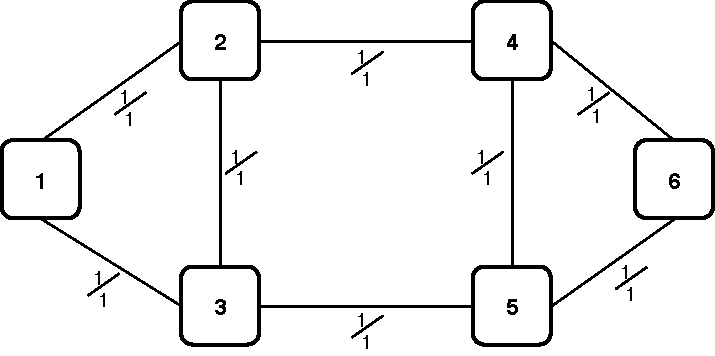
\includegraphics[width=11cm]{sdf/ilp/opaque_survivability/figures/physical_topology}
\caption{Opaque without survivability in medium scenario: physical topology after dimensioning.}
\label{physical_medium}
\end{figure}

\begin{figure}[h!]
\centering
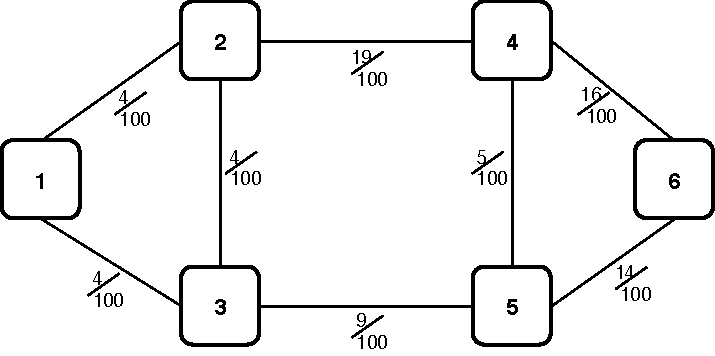
\includegraphics[width=11cm]{sdf/ilp/opaque_survivability/figures/optical_topology_medium}
\caption{Opaque without survivability in medium scenario: optical topology after dimensioning.}
\label{optical_medium}
\end{figure}

We can see the number of optical channels calculated using \ref{Capex_Link} and \ref{Capex} and the number of amplifiers for each link calculated using \ref{Capex_amplifiers} in table \ref{link_opaque_surv_ref_medium}.
\begin{table}[h!]
\centering
\begin{tabular}{|| c | c | c ||}
 \hline
 \multicolumn{3}{|| c ||}{Information regarding links} \\
 \hline
 \hline
 Bidirectional Link & Optical Channels & Amplifiers\\
 \hline
 Node 1 <-> Node 2 & 4 & 4 \\
 Node 1 <-> Node 3 & 4 & 6 \\
 Node 2 <-> Node 3 & 4 & 0 \\
 Node 2 <-> Node 4 & 19 & 6 \\
 Node 3 <-> Node 5 & 9 & 8 \\
 Node 4 <-> Node 5 & 5 & 1 \\
 Node 4 <-> Node 6 & 16 & 7 \\
 Node 5 <-> Node 6 & 14 & 3 \\
 \hline
\end{tabular}
\caption{Table with information regarding links for opaque mode without survivability in medium scenario.}
\label{link_opaque_surv_ref_medium}
\end{table}
\newpage
Also we can see the resulting nodal degree at the physical layer, the number of line ports using \ref{EXC_pexc1_opaque} and the number of tributary ports using \ref{EXC_pexc2_opaque} for each node in table \ref{node_opaque_surv_ref_medium}.

\begin{table}[h!]
\centering
\begin{tabular}{|| c | c | c | c ||}
 \hline
 \multicolumn{4}{|| c ||}{Information regarding nodes} \\
 \hline
 \hline
 Node & Resulting Nodal Degree & Line Ports & Tributary Ports\\
 \hline
 1 & 2 & 8 & 290 \\
 2 & 3 & 27 & 230 \\
 3 & 3 & 17 & 180 \\
 4 & 3 & 40 & 200 \\
 5 & 3 & 28 & 240 \\
 6 & 2 & 30 & 220 \\
\hline
\end{tabular}
\caption{Table with information regarding nodes for opaque mode without survivability in medium scenario.}
\label{node_opaque_surv_ref_medium}
\end{table}

Once again, through the information obtained previously on the nodes we can now create tables with detailed information about each node.\\

\begin{table}[h!]
\centering
\begin{tabular}{|| c | c | c ||}
 \hline
 \multicolumn{3}{|| c ||}{Detailed description of Node 1} \\
 \hline
 \hline
  & Number of total demands & bit rate \\ \hline
\multirow{3}{*}{290 tributary ports} & 130 & ODU0 \\
 & 130 & ODU1 \\
 & 30 & ODU2 \\
 \hline
 \hline
  & Node <-- Optical Channels --> Node & bit rate \\ \hline
\multirow{2}{*}{8 line ports} & 1  <---- 4 ---->  2 & \multirow{2}{*}{100 Gbtis/s} \\
 & 1  <---- 4 ----> 3 & \\
\hline
\end{tabular}
\caption{Opaque without survivability in medium scenario: detailed description of node 1. The number of demands is distributed to the various destination nodes, this distribution can be observed in section \ref{medium_traffic_scenario}.}
\end{table}

\begin{table}[h!]
\centering
\begin{tabular}{|| c | c | c ||}
 \hline
 \multicolumn{3}{|| c ||}{Detailed description of Node 2} \\
 \hline
 \hline
  & Number of total demands & bit rate \\ \hline
\multirow{5}{*}{230 tributary ports} & 110 & ODU0 \\
 & 70 & ODU1 \\
 & 20 & ODU2 \\
 & 20 & ODU3 \\
 & 10 & ODU4 \\
 \hline
 \hline
  & Node <-- Optical Channels --> Node & bit rate \\ \hline
 \multirow{3}{*}{27 line ports} & 2  <---- 4 ---->  1 & \multirow{3}{*}{100 Gbtis/s}\\
 & 2  <---- 4 ---->  3 & \\
 & 2  <---- 19 ---->  4 & \\
\hline
\end{tabular}
\caption{Opaque without survivability in medium scenario: detailed description of node 2. The number of demands is distributed to the various destination nodes, this distribution can be observed in section \ref{medium_traffic_scenario}.}
\end{table}

\newpage
\begin{table}[h!]
\centering
\begin{tabular}{|| c | c | c ||}
 \hline
 \multicolumn{3}{|| c ||}{Detailed description of Node 3} \\
 \hline
 \hline
  & Number of total demands & bit rate \\ \hline
\multirow{4}{*}{180 tributary ports} & 70 & ODU0 \\
 & 60 & ODU1\\
 & 30 & ODU2\\
 & 20 & ODU3\\
 \hline
 \hline
  & Node <-- Optical Channels --> Node & bit rate \\ \hline
 \multirow{3}{*}{17 line ports} & 3  <---- 4 ---->  1 & \multirow{3}{*}{100 Gbtis/s}\\
 & 3  <---- 4 ---->  2 & \\
 & 3  <---- 9 ---->  5 & \\
\hline
\end{tabular}
\caption{Opaque without survivability in medium scenario: detailed description of node 3. The number of demands is distributed to the various destination nodes, this distribution can be observed in section \ref{medium_traffic_scenario}.}
\end{table}

\begin{table}[h!]
\centering
\begin{tabular}{|| c | c | c ||}
 \hline
 \multicolumn{3}{|| c ||}{Detailed description of Node 4} \\
 \hline
 \hline
  & Number of total demands & bit rate \\ \hline
\multirow{3}{*}{200 tributary ports} & 70 & ODU0 \\
 & 100 & ODU1 \\
 & 30 & ODU2 \\
 \hline
 \hline
  & Node <-- Optical Channels --> Node & bit rate \\ \hline
\multirow{3}{*}{40 line ports} & 4  <---- 19 ---->  2 & \multirow{3}{*}{100 Gbtis/s}\\
 & 4  <---- 5 ---->  5 & \\
 & 4  <---- 16 ---->  6 & \\
\hline
\end{tabular}
\caption{Opaque without survivability in medium scenario: detailed description of node 4. The number of demands is distributed to the various destination nodes, this distribution can be observed in section \ref{medium_traffic_scenario}.}
\end{table}

\begin{table}[h!]
\centering
\begin{tabular}{|| c | c | c ||}
 \hline
 \multicolumn{3}{|| c ||}{Detailed description of Node 5} \\
 \hline
 \hline
  & Number of total demands & bit rate \\ \hline
\multirow{5}{*}{240 tributary ports} & 140 & ODU0 \\
 & 40 & ODU1 \\
 & 40 & ODU2 \\
 & 10 & ODU3 \\
 & 10 & ODU4 \\
 \hline
 \hline
  & Node <-- Optical Channels --> Node & bit rate \\ \hline
 \multirow{3}{*}{28 line ports} & 5  <---- 9 ---->  3 & \multirow{3}{*}{100 Gbtis/s} \\
 & 5  <---- 5 ---->  4 & \\
 & 5  <---- 14 ---->  6 & \\
\hline
\end{tabular}
\caption{Opaque without survivability in medium scenario: detailed description of node 5. The number of demands is distributed to the various destination nodes, this distribution can be observed in section \ref{medium_traffic_scenario}.}
\end{table}

\newpage
\begin{table}[h!]
\centering
\begin{tabular}{|| c | c | c ||}
 \hline
 \multicolumn{3}{|| c ||}{Detailed description of Node 6} \\
 \hline
 \hline
  & Number of total demands & bit rate \\ \hline
\multirow{5}{*}{220 tributary ports} & 80 & ODU0 \\
 & 100 & ODU1 \\
 & 10 & ODU2 \\
 & 10 & ODU3 \\
 & 20 & ODU4 \\
 \hline
 \hline
  & Node <-- Optical Channels --> Node & bit rate \\ \hline
 \multirow{2}{*}{30 line ports} & 6  <---- 16 ---->  4 & \multirow{2}{*}{100 Gbtis/s} \\
 & 6  <---- 14 ---->  5 & \\
\hline
\end{tabular}
\caption{Opaque without survivability in medium scenario: detailed description of node 6. The number of demands is distributed to the various destination nodes, this distribution can be observed in section \ref{medium_traffic_scenario}.}
\end{table}

\vspace{11pt}
In next step let's focus on the routing information. These paths are bidirectional so the path from one node to another is the same path in the opposite direction. In table \ref{path_opaque_surv_ref_medium} we can see all the routing obtained for all nodes.\\

\begin{table}[h!]
\centering
\begin{tabular}{|| c | c | c | c | c | c | c | c ||}
 \hline
 \multicolumn{8}{|| c ||}{Routing} \\
 \hline
 \hline
 o & d & Links & ODU0 & ODU1 & ODU2 & ODU3 & ODU4 \\
 \hline
 1 & 2 & \{(1,2)\} & 50 & 20 & 10 & 0 & 0 \\ \hline
 1 & 3 & \{(1,3)\} & 10 & 40 & 10 & 0 & 0\\ \hline
 1 & 4 & \{(1,2),(2,4)\} & 30 & 20 & 10 & 0 & 0\\ \hline
 1 & 5 & \{(1,3),(3,5)\} & 10 & 0 & 0 & 0 & 0\\ \hline
 1 & 6 & \{(1,3),(3,5),(5,6)\} & 30 & 50 & 0 & 0 & 0\\ \hline
 2 & 3 & \{(2,3)\} & 0 & 0 & 0 & 10 & 0 \\ \hline
 2 & 4 & \{(2,4)\} & 10 & 30 & 0 & 0 & 0\\ \hline
 2 & 5 & \{(2,4),(4,5)\} & 50 & 10 & 10 & 0 & 0 \\ \hline
 2 & 6 & \{(2,4),(4,6)\} & 0 & 10 & 0 & 10 & 10 \\ \hline
 3 & 4 & \{(3,5),(5,4)\} & 10 & 10 & 10 & 0 & 0 \\ \hline
 3 & 5 & \{(3,5)\} & 40 & 10 & 10 & 10 & 0 \\ \hline
 3 & 6 & \{(3,5),(5,6)\} & 10 & 0 & 0 & 0 & 0\\ \hline
 4 & 5 & \{(4,5)\} & 10 & 10 & 10 & 0 & 0\\ \hline
 4 & 6 & \{(4,6)\} & 10 & 30 & 0 & 0 & 0\\ \hline
 5 & 6 & \{(5,6)\} & 30 & 10 & 10 & 0 & 10\\
 \hline
\end{tabular}
\caption{Opaque without survivability in medium scenario: table with description of demands routing. We are assuming that between a pair of nodes all demands follow the same route.}
\label{path_opaque_surv_ref_medium}
\end{table}

Finally through the table \ref{scriptopaque_surv_ref_medium} we can see the CAPEX result for this model. This value is obtained using equation \ref{ILPOpaque_CAPEX} and all of the constraints mentioned above.\\
\newpage
\begin{table}[h!]
\centering
\begin{tabular}{||c|c|c|c|c|c|c||}
 \hline
 \multicolumn{7}{||c||}{CAPEX of the Network} \\
 \hline
 \hline
 \multicolumn{3}{||c|}{ } & Quantity & Unit Price & Cost & Total \\
 \hline
 \multirow{3}{*}{\makecell{Link \\ Cost}} & \multicolumn{2}{ c |}{OLTs} & 16 & 15 000 \euro & 240 000 \euro & \multirow{3}{*}{75 520 000 \euro} \\ \cline{2-6}
 & \multicolumn{2}{c|}{100 Gbits/s Transceivers} & 150 & 5 000 \euro/Gbit/s & 75 000 000 \euro & \\ \cline{2-6}
 & \multicolumn{2}{c|}{Amplifiers} & 70 & 4 000 \euro & 280 000 \euro & \\
 \hline
 \multirow{9}{*}{\makecell{Node \\ Cost}} & \multirow{7}{*}{Electrical} & EXCs & 6 & 10 000 \euro & 60 000 \euro & \multirow{9}{*}{15 085 900 \euro} \\ \cline{3-6}
 & & ODU0 Ports & 600 & 10 \euro/port & 6 000 \euro & \\ \cline{3-6}
 & & ODU1 Ports & 500 & 15 \euro/port & 7 500 \euro & \\ \cline{3-6}
 & & ODU2 Ports & 160 & 30 \euro/port & 4 800 \euro & \\ \cline{3-6}
 & & ODU3 Ports & 60 & 60 \euro/port & 3 600 \euro & \\ \cline{3-6}
 & & ODU4 Ports & 40 & 100 \euro/port & 4 000 \euro & \\ \cline{3-6}
 & & Line Ports & 150 & 100 000 \euro/port & 15 000 000 \euro & \\ \cline{2-6}
 & \multirow{2}{*}{Optical} & OXCs & 0 & 20 000 \euro & 0 \euro & \\ \cline{3-6}
 & & Ports & 0 & 2 500 \euro/port & 0 \euro & \\
 \hline
 \multicolumn{6}{||c|}{Total Network Cost} & 90 605 900 \euro \\
\hline
\end{tabular}
\caption{Opaque without survivability in medium scenario: detailed description of CAPEX for this scenario.}
\label{scriptopaque_surv_ref_medium}
\end{table}

\textbf{High Traffic Scenario:}\\

In a first phase, we will show the resulting physical and optical topology. These topologies are based on the allowed topologies referred to in the model description and also taking into account the logical topology for all ODUs mentioned in the section \ref{high_traffic_scenario}.\\

\begin{figure}[h!]
\centering
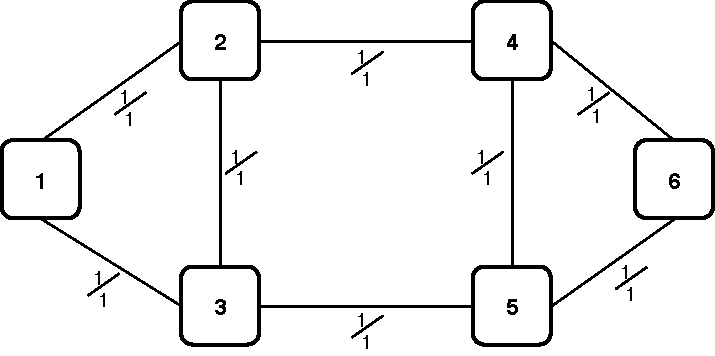
\includegraphics[width=11cm]{sdf/ilp/opaque_survivability/figures/physical_topology}
\caption{Opaque without survivability in high scenario: physical topology after dimensioning.}
\label{physical_high}
\end{figure}
\newpage
\begin{figure}[h!]
\centering
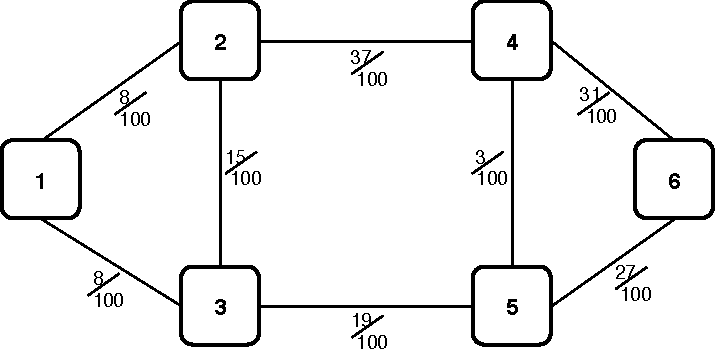
\includegraphics[width=11cm]{sdf/ilp/opaque_survivability/figures/optical_topology_high}
\caption{Opaque without survivability in high scenario: optical topology after dimensioning.}
\label{optical_high}
\end{figure}

In table \ref{link_opaque_surv_ref_high} we can see the number of optical channels calculated using \ref{Capex_Link} and \ref{Capex} and the number of amplifiers for each link calculated using \ref{amplifiers}.

\begin{table}[h!]
\centering
\begin{tabular}{|| c | c | c ||}
 \hline
 \multicolumn{3}{|| c ||}{Information regarding links} \\
 \hline
 \hline
 Bidirectional Link & Optical Channels & Amplifiers\\
 \hline
 Node 1 <-> Node 2 & 8 & 4 \\
 Node 1 <-> Node 3 & 8 & 6 \\
 Node 2 <-> Node 3 & 15 & 0 \\
 Node 2 <-> Node 4 & 37 & 6 \\
 Node 3 <-> Node 5 & 19 & 8 \\
 Node 4 <-> Node 5 & 3 & 1 \\
 Node 4 <-> Node 6 & 31 & 7 \\
 Node 5 <-> Node 6 & 27 & 3 \\
 \hline
\end{tabular}
\caption{Table with information regarding links for opaque mode without survivability in high scenario.}
\label{link_opaque_surv_ref_high}
\end{table}

In table \ref{node_opaque_surv_ref_high} we can see the resulting nodal degree at the physical layer, calculated based on the number of connections that the node in question performs, the number of line ports calculated using \ref{EXC_pexc1_opaque} and the number of tributary ports calculated using \ref{EXC_pexc2_opaque} for each node.

\begin{table}[h!]
\centering
\begin{tabular}{|| c | c | c | c ||}
 \hline
 \multicolumn{4}{|| c ||}{Information regarding nodes} \\
 \hline
 \hline
 Node & Resulting Nodal Degree & Line Ports & Tributary Ports\\
 \hline
 1 & 2 & 16 & 580 \\
 2 & 3 & 60 & 460 \\
 3 & 3 & 42 & 360 \\
 4 & 3 & 71 & 400 \\
 5 & 3 & 49 & 480 \\
 6 & 2 & 58 & 440 \\
\hline
\end{tabular}
\caption{Table with information regarding nodes for opaque mode without survivability in high scenario.}
\label{node_opaque_surv_ref_high}
\end{table}
\newpage
In each table mentioned next with detailed information we can see how many ports are connected to a given node and its bit rate (in relation to the line ports) and how many ports are assigned to each different bit rate (in relation to the tributary ports).

\begin{table}[h!]
\centering
\begin{tabular}{|| c | c | c ||}
 \hline
 \multicolumn{3}{|| c ||}{Detailed description of Node 1} \\
 \hline
 \hline
  & Number of total demands & bit rate \\ \hline
\multirow{3}{*}{580 tributary ports} & 260 & ODU0 \\
 & 260 & ODU1 \\
 & 60 & ODU2 \\
 \hline
 \hline
  & Node <-- Optical Channels --> Node & bit rate \\ \hline
\multirow{2}{*}{16 line ports} & 1  <---- 8 ---->  2 & \multirow{2}{*}{100 Gbtis/s} \\
 & 1  <---- 8 ---->  3 & \\
\hline
\end{tabular}
\caption{Opaque without survivability in high scenario: detailed description of node 1. The number of demands is distributed to the various destination nodes, this distribution can be observed in section \ref{high_traffic_scenario} .}
\end{table}

\begin{table}[h!]
\centering
\begin{tabular}{|| c | c | c ||}
 \hline
 \multicolumn{3}{|| c ||}{Detailed description of Node 2} \\
 \hline
 \hline
  & Number of total demands & bit rate \\ \hline
\multirow{5}{*}{460 tributary ports} & 220 & ODU0 \\
 & 140 & ODU1 \\
 & 40 & ODU2 \\
 & 40 & ODU3 \\
 & 20 & ODU4 \\
\hline
\hline
 & Node <-- Optical Channels --> Node & bit rate \\ \hline
 \multirow{3}{*}{60 line ports} & 2  <---- 8 ---->  1 & \multirow{3}{*}{100 Gbtis/s}\\
 & 2  <---- 15 ---->  3 & \\
 & 2  <---- 37 ---->  4 & \\
 \hline
\end{tabular}
\caption{Opaque without survivability in high scenario: detailed description of node 2. The number of demands is distributed to the various destination nodes, this distribution can be observed in section \ref{high_traffic_scenario}.}
\end{table}

\begin{table}[h!]
\centering
\begin{tabular}{|| c | c | c ||}
 \hline
 \multicolumn{3}{|| c ||}{Detailed description of Node 3} \\
 \hline
 \hline
  & Number of total demands & bit rate \\ \hline
\multirow{4}{*}{360 tributary ports} & 140 & ODU0 \\
 & 120 & ODU1\\
 & 60 & ODU2\\
 & 40 & ODU3\\
 \hline
 \hline
  & Node <-- Optical Channels --> Node & bit rate \\ \hline
 \multirow{3}{*}{42 line ports} & 3  <---- 8 ---->  1 & \multirow{3}{*}{100 Gbtis/s}\\
 & 3  <---- 15 ---->  2 & \\
 & 3  <---- 19 ---->  5 & \\
\hline
\end{tabular}
\caption{Opaque without survivability in high scenario: detailed description of node 3. The number of demands is distributed to the various destination nodes, this distribution can be observed in section \ref{high_traffic_scenario}.}
\end{table}
\newpage
\begin{table}[h!]
\centering
\begin{tabular}{|| c | c | c ||}
 \hline
 \multicolumn{3}{|| c ||}{Detailed description of Node 4} \\
 \hline
 \hline
  & Number of total demands & bit rate \\ \hline
\multirow{3}{*}{400 tributary ports} & 140 & ODU0 \\
 & 200 & ODU1 \\
 & 60 & ODU2 \\
 \hline
 \hline
  & Node <-- Optical Channels --> Node & bit rate \\ \hline
\multirow{3}{*}{71 line ports} & 4  <---- 37 ---->  2 & \multirow{3}{*}{100 Gbtis/s}\\
 & 4  <---- 3 ---->  5 & \\
 & 4  <---- 31 ---->  6 & \\
\hline
\end{tabular}
\caption{Opaque without survivability in high scenario: detailed description of node 4. The number of demands is distributed to the various destination nodes, this distribution can be observed in section \ref{high_traffic_scenario}.}
\end{table}

\begin{table}[h!]
\centering
\begin{tabular}{|| c | c | c ||}
 \hline
 \multicolumn{3}{|| c ||}{Detailed description of Node 5} \\
 \hline
 \hline
  & Number of total demands & bit rate \\ \hline
\multirow{5}{*}{480 tributary ports} & 280 & ODU0 \\
 & 80 & ODU1 \\
 & 80 & ODU2 \\
 & 20 & ODU3 \\
 & 20 & ODU4 \\
 \hline
 \hline
  & Node <-- Optical Channels --> Node & bit rate \\ \hline
 \multirow{3}{*}{49 line ports} & 5  <---- 19 ---->  3 & \multirow{3}{*}{100 Gbtis/s} \\
 & 5  <---- 3 ---->  4 & \\
 & 5  <---- 27 ---->  6 & \\
\hline
\end{tabular}
\caption{Opaque without survivability in high scenario: detailed description of node 5. The number of demands is distributed to the various destination nodes, this distribution can be observed in section \ref{high_traffic_scenario}.}
\end{table}

\begin{table}[h!]
\centering
\begin{tabular}{|| c | c | c ||}
 \hline
 \multicolumn{3}{|| c ||}{Detailed description of Node 6} \\
 \hline
 \hline
  & Number of total demands & bit rate \\ \hline
\multirow{5}{*}{440 tributary ports} & 160 & ODU0 \\
 & 200 & ODU1 \\
 & 20 & ODU2 \\
 & 20 & ODU3 \\
 & 40 & ODU4 \\
 \hline
 \hline
  & Node <-- Optical Channels --> Node & bit rate \\ \hline
 \multirow{2}{*}{58 line ports} & 6  <---- 31 ---->  4 & \multirow{2}{*}{100 Gbtis/s} \\
 & 6  <---- 27 ---->  5 & \\
\hline
\end{tabular}
\caption{Opaque without survivability in high scenario: detailed description of node 6. The number of demands is distributed to the various destination nodes, this distribution can be observed in section \ref{high_traffic_scenario}.}
\end{table}

\newpage
Next step let's focus on the routing information. These paths are bidirectional so the path from one node to another is the same path in the opposite direction. In table \ref{path_opaque_surv_ref_high} we can see all the routing obtained for all nodes.

\begin{table}[h!]
\centering
\begin{tabular}{|| c | c | c | c | c | c | c | c ||}
 \hline
 \multicolumn{8}{|| c ||}{Routing} \\
 \hline
 \hline
 o & d & Links & ODU0 & ODU1 & ODU2 & ODU3 & ODU4 \\
 \hline
 1 & 2 & \{(1,2)\} & 100 & 40 & 20 & 0 & 0 \\ \hline
 1 & 3 & \{(1,3)\} & 20 & 80 & 20 & 0 & 0\\ \hline
 1 & 4 & \{(1,2),(2,4)\} & 60 & 40 & 20 & 0 & 0\\ \hline
 1 & 5 & \{(1,3),(3,5)\} & 20 & 0 & 0 & 0 & 0\\ \hline
 1 & 6 & \{(1,3),(3,5),(5,6)\} & 60 & 100 & 0 & 0 & 0\\ \hline
 2 & 3 & \{(2,3)\} & 0 & 0 & 0 & 20 & 0 \\ \hline
 2 & 4 & \{(2,4)\} & 20 & 60 & 0 & 0 & 0\\ \hline
 2 & 5 & \{(2,3),(3,5)\} & 100 & 20 & 20 & 0 & 0 \\ \hline
 2 & 6 & \{(2,4),(4,6)\} & 0 & 20 & 0 & 20 & 20 \\ \hline
 3 & 4 & \{(3,2),(2,4)\} & 20 & 20 & 20 & 0 & 0 \\ \hline
 3 & 5 & \{(3,5)\} & 80 & 20 & 20 & 20 & 0 \\ \hline
 3 & 6 & \{(3,5),(5,6)\} & 20 & 0 & 0 & 0 & 0\\ \hline
 4 & 5 & \{(4,5)\} & 20 & 20 & 20 & 0 & 0\\ \hline
 4 & 6 & \{(4,6)\} & 20 & 60 & 0 & 0 & 0\\ \hline
 5 & 6 & \{(5,6)\} & 60 & 20 & 20 & 0 & 20\\
 \hline
\end{tabular}
\caption{Opaque without survivability in high scenario: description of demands routing. We are assuming that between a pair of nodes all demands follow the same route.}
\label{path_opaque_surv_ref_high}
\end{table}

Finally and most importantly through table \ref{scriptopaque_surv_ref_high} we can see the CAPEX result for this model. This value is obtained using equation \ref{ILPOpaque_CAPEX} and all of the constraints mentioned above.

\begin{table}[h!]
\centering
\begin{tabular}{||c|c|c|c|c|c|c||}
 \hline
 \multicolumn{7}{||c||}{CAPEX of the Network} \\
 \hline
 \hline
 \multicolumn{3}{||c|}{ }&Quantity&Unit Price&Cost&Total \\
 \hline
 \multirow{3}{*}{\makecell{Link \\ Cost}}&\multicolumn{2}{c|}{OLTs}&16&15 000 \euro&240 000 \euro&\multirow{3}{*}{148 520 000 \euro}\\ \cline{2-6}
 &\multicolumn{2}{c|}{100 Gbits/s Transceivers}&296&5 000 \euro/Gbit/s&148 000 000 \euro&\\ \cline{2-6}
 &\multicolumn{2}{c|}{Amplifiers}&70&4 000 \euro&280 000 \euro&\\
 \hline
 \multirow{9}{*}{\makecell{Node \\ Cost}}&\multirow{7}{*}{Electrical}&EXCs&6&10 000 \euro&60 000 \euro&\multirow{9}{*}{29 711 800 \euro}\\ \cline{3-6}
 & &ODU0 Ports&1 200&10 \euro/port&12 000 \euro&\\ \cline{3-6}
 & &ODU1 Ports&1 000&15 \euro/port&15 000 \euro&\\ \cline{3-6}
 & &ODU2 Ports&320&30 \euro/port&9 600 \euro&\\ \cline{3-6}
 & &ODU3 Ports&120&60 \euro/port&7 200 \euro&\\ \cline{3-6}
 & &ODU4 Ports&80&100 \euro/port&8 000 \euro&\\ \cline{3-6}
 & &Line Ports&296&100 000 \euro/port&29 600 000 \euro&\\ \cline{2-6}
 &\multirow{2}{*}{Optical}&OXCs&0&20 000 \euro&0 \euro&\\ \cline{3-6}
 & &Ports&0&2 500 \euro/port&0 \euro&\\
 \hline
 \multicolumn{6}{||c|}{Total Network Cost}&178 231 800 \euro \\
\hline
\end{tabular}
\caption{Opaque without survivability in high scenario: detailed description of CAPEX for this scenario.}
\label{scriptopaque_surv_ref_high}
\end{table}

\newpage
\subsection{Conclusions}

Once we have obtained the results for all the scenarios we will now draw some conclusions about these results. For a better analysis of the results will be created the table \ref{table_comparative_opaque_surv} with the number of line ports, tributary ports and transceivers because they are important values for the cost of CAPEX, the cost of links, the cost of nodes and finally the cost of CAPEX.\\

\begin{table}[h!]
\centering
\begin{tabular}{| c | c | c | c |}
 \hline
  & Low Traffic & Medium Traffic  & High Traffic \\
 \hline\hline
 Traffic (Gbit/s) & 500 & 5 000 & 10 000 \\ \hline
 Bidirectional Links used & 6 & 8 & 8 \\ \hline
 Number of Line ports & 18 & 150 & 296 \\ \hline
 Number of Tributary ports & 136 & 1 360 & 2 720 \\ \hline
 Number of Transceivers & 18 & 150 & 296 \\ \hline
 Link Cost & 9 404 000 \euro & 75 520 000 \euro & 148 520 000 \euro \\ \hline
 Node Cost & 1 862 590 \euro & 15 085 900 \euro & 29 711 800 \euro \\ \hline
 CAPEX & \textbf{11 266 590 \euro} & \textbf{90 605 900 \euro} & \textbf{178 231 800 \euro} \\ \hline
 CAPEX/Gbit/s & \textbf{22 533 \euro/Gbit/s} & \textbf{18 121 \euro/Gbit/s} & \textbf{17 823 \euro/Gbit/s}\\
 \hline
\end{tabular}
\caption{Opaque without survivability: table with the various CAPEX values obtained in the different traffic scenarios.}
\label{table_comparative_opaque_surv}
\end{table}

Looking at the previous table we can make some comparisons between the several scenarios:

\begin{itemize}
  \item Low traffic scenario uses less links than the other two scenarios. This happens because as it has low traffic it is possible to carry it throughout the network without having to use all available links;
  \item Comparing the low traffic scenario with the others we can see that despite having an increase of factor ten (medium scenario) and factor twenty (high scenario) the same increase does not occur in the final cost (it is lower). This happens because the number of transceivers is smaller than expected (medium scenario would be expected 180 and high scenario would be expected 360);
  \item Comparing the medium traffic scenario with the high traffic scenario we can see that the increase of the factor is double and in the final cost this factor is very close but still inferior. Again this happens because the number of transceivers is lower but very close to the expected (high scenario would be expected 300);
  \item Comparing the cost with traffic we can see that as traffic increases, the cost per traffic decreases. Soon we can conclude that it becomes more expensive a scenario of low traffic than a scenario of high traffic.
\end{itemize}


